\documentclass{article}


% if you need to pass options to natbib, use, e.g.:
%     \PassOptionsToPackage{numbers, compress}{natbib}
% before loading neurips_2023


% ready for submission
\usepackage[final, nonatbib]{neurips_2023}


% to compile a preprint version, e.g., for submission to arXiv, add add the
% [preprint] option:
%     \usepackage[preprint]{neurips_2023}


% to compile a camera-ready version, add the [final] option, e.g.:
%     \usepackage[final]{neurips_2023}


% to avoid loading the natbib package, add option nonatbib:
%    \usepackage[nonatbib]{neurips_2023}


\usepackage[utf8]{inputenc} % allow utf-8 input
\usepackage[T1]{fontenc}    % use 8-bit T1 fonts
\usepackage{hyperref}       % hyperlinks
\usepackage{url}            % simple URL typesetting
\usepackage{booktabs}       % professional-quality tables
\usepackage{amsfonts}       % blackboard math symbols
\usepackage{nicefrac}       % compact symbols for 1/2, etc.
\usepackage{microtype}      % microtypography
\usepackage{xcolor}         % colors

\usepackage[spanish, es-tabla]{babel}

\usepackage[pdftex]{graphicx}
\usepackage{pgf}
\usepackage{subcaption}
\graphicspath{{./graphs/}}

%% biblatex
\usepackage[style = numeric, backend = biber, sorting = none, doi = false, isbn = false, url = true]{biblatex}
% \usepackage[defernumbers = true, style = numeric, backend = biber, sorting = none, doi = false, isbn = false, url = true]{biblatex}
% \usepackage[style = numeric, backend = biber, sorting = none]{biblatex}    % REFERENCIAS como section
\AtEveryBibitem{
    \clearfield{urlyear}
    \clearfield{urlmonth}
} % Do not show the "(visited on <date>)" on the references
\DefineBibliographyStrings{spanish}{}
\usepackage{csquotes}
\addbibresource{./dmcyt.bib}
\renewcommand*{\bibfont}{\fontsize{9}{12}\selectfont}



\title{Grafos en neurociencias (pre TP2)}

\author{
  Víctor A.~Bettachini\\ %\thanks{Use footnote for providing further information about author (webpage, alternative address)---\emph{not} for acknowledging funding agencies.} \\
  Datamining en ciencia y tecnología 2023\\
  Especialización en Explotación de Datos y Descubrimiento del Conocimiento\\
  \texttt{bettachini@gmail.com}
}


\begin{document}


\maketitle


\begin{abstract}
?
\end{abstract}


% Enunciado
% Se sugiere realizar la entrega en formato latex, pero en este caso va a ser optativo (en el TP ya es obligatorio, sugerimos que lo usen de práctica). Pueden acceder a formatos de distintas conferencias a través de Overleaf, en particular les sugerimos el formato de NeurIPS que es una de las conferencias más importantes en IA.
% Se sugiere un máx de 4 carillas (mín 2), no se debe incluir código a menos que sea algo esencial que hayan desarrollado ustedes (es preferible en este caso incluir el pseudo-código). Aclaración: No vamos a corregir código en la entrega.
% El pre TP es individual.


% \section{Introducción}

\section{Materiales y métodos}

\paragraph{Datos}
Se hace uso de datos producto de la medición de la señal de resonancia magnética funcional (fMRI).
Definidos 116 volúmenes de interés del cerebro en términos de su activación \cite{tzourio-mazoyer_automated_2002}, se publicaron coeficientes de correlación lineal entre sus medias en distintos segmentos temporales \cite{tagliazucchi_large-scale_2013}.
Con estos datos se generó una matríz de correlación, y a partir de la misma los grafos analizados en este trabajo.


\paragraph{Recurso informático} 
Un cuaderno (notebook) Jupyter provisto por los docentes en el sitio web denominado ``Campus'' \cite{kamienkowski_curso_2023} es la plantilla donde se escribió código en lenguaje Python.
Este explotó funciones de las biblioteca NetworkX \cite{hagberg_exploring_2008}.



\subsection{Preprocesamiento de los datos}
% Cada actividad realizada se describe bajo los titulos que figuran en el enunciado del trabajo práctico publicado en el

\paragraph{Carga del conjunto de datos} 
Los archivos provistos corresponden a los estadíos de sueño N1, N2, N3 y despierto (W) para 18 sujetos.
Estos estuvieron acompañados de una tabla que describe la denominacion y  ubicación espacial las regiones en que se parcializó el cerebro.



\section{Resultados}

\subsection{Manipulación de datos}

\paragraph{Matriz de correlación}
La matriz de adyacencia pesada que muestra la figura \ref{fg:matriz_correlación_pesada} corresponde a la condición de despierto para el sujeto número 2.

Una medida que caracteriza un grafo es la densidad, $\delta$, definida como la razón entre los enlaces presentes sobre todos los posibles en el grafo.
Para convertir la matriz en una de adyacencia binaria con una densidad de enlaces \(\delta = 0.8\) se discriminaron sus pesos con un umbral \(0.77997\) obteníendose la matriz que muestra la figura \ref{fg:matriz_correlación_binaria}.

\begin{figure}[ht]
	\centering
	\begin{subfigure}[b]{0.39\textwidth}
		\includegraphics[width= \linewidth]{matriz_correlación}
		\caption{Pesada}
		\label{fg:matriz_correlación_pesada}
	\end{subfigure}
	\begin{subfigure}[b]{0.33\textwidth}
		\includegraphics[width= \linewidth]{matriz_correlación_binaria}
		\caption{Binaria}
		\label{fg:matriz_correlación_binaria}
	\end{subfigure}
	\caption{Matrices de correlación de las medias de las señales de las regiones parcializadas para el sujeto número 2 despierto. 
	}
	\label{fg:matriz_correlación}
\end{figure}


\paragraph{Grafo de la matriz de adyacencia binaria}
No es totalmente conectado. Hay tres componentes conectadas de 92, 5 y 2 nodos en tanto que los 17 restantes están aislados.
La distancia mínima entre nodos contabiliza cuantos intermedios deben atravesarse para ir de un nodo a otro.
Esta medida para los aislados no tiene sentido, por lo en este grafo no puede obtenerse una distancia media $d$ a lo fines de tener una media de que tan ``conectado'' se presenta el grafo.
Una medida númerica alternativa la provee la densidad.
Para el conjunto, no conectado, este valor parece bajo, $\approx 8\%$.
Y en el componente mayoritario, el de 92 nodos, este valor apenas se incrementa hasta un $\approx 12\%$. 


\paragraph{Eficiencia de conectividad}
La distancia mínima entre nodos contabiliza cuantos intermedios deben atravesarse para ir de un nodo a otro.
Un promedio de la inversa de esta distancia es una medida de la eficiencia de conectividad global del grafo, que para este caso resultó ser $\approx 0.389$.


\paragraph{Distribución de grado}
El número de enlaces por nodo, o grado $k$, se distribuye en forma dispar.
De un total de $534$ enlaces el grado mayor resultó $k_\textnormal{máx} = 30$, y un relativamente alto promedio $\langle k \rangle \approx 9.207$ aunque no hay que olvidar que no participan aquí los nodos aislados.
El histograma de $k$ que muestra la figura \ref{fg:hist_k} que este $\langle k \rangle$ es representativo de la distribución.

En una medida similar a la densidad que cuenta la proporción de enlaces sobre los posibles puede hacerse algo similar calculando la proporción de cuantos de los posibles enlaces entre primeros vecinos efectivamente se realizan.
Esto se denomina coeficiente de agrupamiento (clustering) por nodo $C_i$, cuyo promedio para este grafo es $\langle C_i \rangle \approx 0.527$. 
Coloreando cada nodo según su $C_i$ y ubicandole por las coordenadas (y,z) en el cerebro se obtiene la figura \ref{fg:clustering}. 

\begin{figure}[ht]
	\centering
	\begin{subfigure}[b]{0.25\textwidth}
		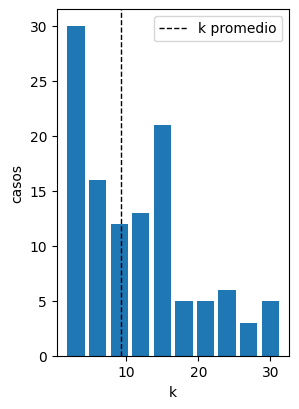
\includegraphics[width= \linewidth]{histograma_k}
		\caption{Histograma para $k$.
		}
		\label{fg:hist_k}
	\end{subfigure}
	\begin{subfigure}[b]{0.7\textwidth}
		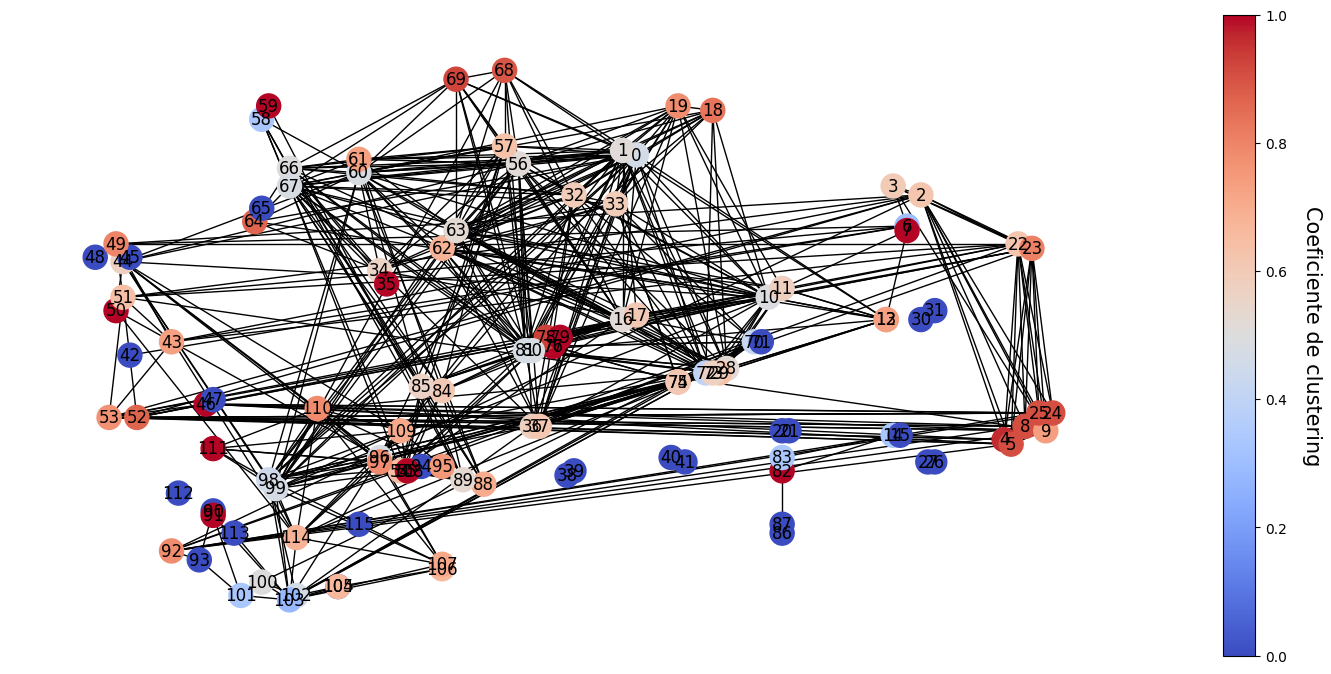
\includegraphics[width= \linewidth]{clustering}
		\caption{número de nodo $i$ y su $C_i$.
		}
		\label{fg:clustering}
	\end{subfigure}
	\caption{Distribución de grado y coeficiente de agrupamiento.
	}
	\label{fg:distribución_de_grado}
\end{figure}


\paragraph{Grafos prototípicos}
Se generaron grafos aleatorios con la misma cantidad de nodos, $n = 116$ que el grafo de la matriz de adyacencia binaria a los fines de encontrar semejanzas y determinar cuál de estos explicaría la la estructura del grafo producto de las mediciones.

El algoritmo de Erdös–Rényi enlaza un par de nodos si una probabilidad al azar supera un umbral \cite[sección 3.2]{albert-laszlo_barabasi_network_2016}.
Estableciendo en función del $\langle k \rangle$ de la red original tal probabilidad como $p = \frac{\langle k \rangle}{n -1}$ se obtuvo una densidad prácticamente idéntica $\delta = 0.0808$ a la de la red original, $0.0801$, con una suma de enlaces, $539$, también muy cercana, $534$. 
El coeficiente de agrupamiento $\langle C_i \rangle = 0.7986$ resulta bastante disímil con el $0.5271$ de la red original.
Esta red azarosa, a diferencia de la original, mostró estar totalmente conectada, como se aprecia en la figura \ref{fg:erdos_renyi}. 
En contrapartida, las redes reales suelen estar particionadas en múltiples componentes conectadas \cite[sección 3.7]{albert-laszlo_barabasi_network_2016}.

Si una red fuera perfectamente regular ytodos los nodos tuvieran idéntica $k$, la distancia mínima entre dos nodos $d$, es decir cuantos intermedios debe atravezarse para enlazar uno con otro, seguiría una dependencia polinomial con $n$.
En las redes reales $d$ presenta una dependencia mucho menor con $n$, con $\log(n)$ de hecho.
Este fenómeno recibe el nombre de ``mundo pequeño'' (small-world) por la sorpresiva poca distancia entre dos cualesquiera nodos de la red.
Asimismo, en las reales, el coeficiente de agrupamiento $C_i$ suele ser más alto que en una red azarosa \cite[sección 3.9]{albert-laszlo_barabasi_network_2016}. 
En respuesta a estas observaciones, Watts y Strogatz extendieron el modelo ordenado con un $k$ regular con un parámetro adicional que determina la probabilidad de que un enlace cambie su enlace hacia otro nodo, generando redes intermedias entre una regular y una azarosa.
El número de enlaces total más cercano al de la red original, $580$, se obtuvo con $k = \mathrm{int}(\langle k \rangle) + 1$. 
Puesto que la $\delta = 0.870$ es insensible al parámetro de reconexión se lo ajustó buscando un $\langle C_i \rangle$ similar al de la red original.
Este fluctua por efectos azarosos pero se logró que este oscilara en torno al $\approx 0.527$ con una probabilidad de reconexión de $0.815$.
Pero la red generada se presenta totalmente conectada y con un aspecto muy diferente a la original, como muestra la figura \ref{fg:watts_strogatz}. 
Se pude generar con el algoritmo de Watts-Strogatz una red con aspecto más similar incrementando la reconexión y así haciendola más azarosa y por tanto a la original, pero el resultante $\langle C_i \rangle$ se aleja del de esta.


\begin{figure}[ht]
	\centering
	\begin{subfigure}[b]{0.32\textwidth}
		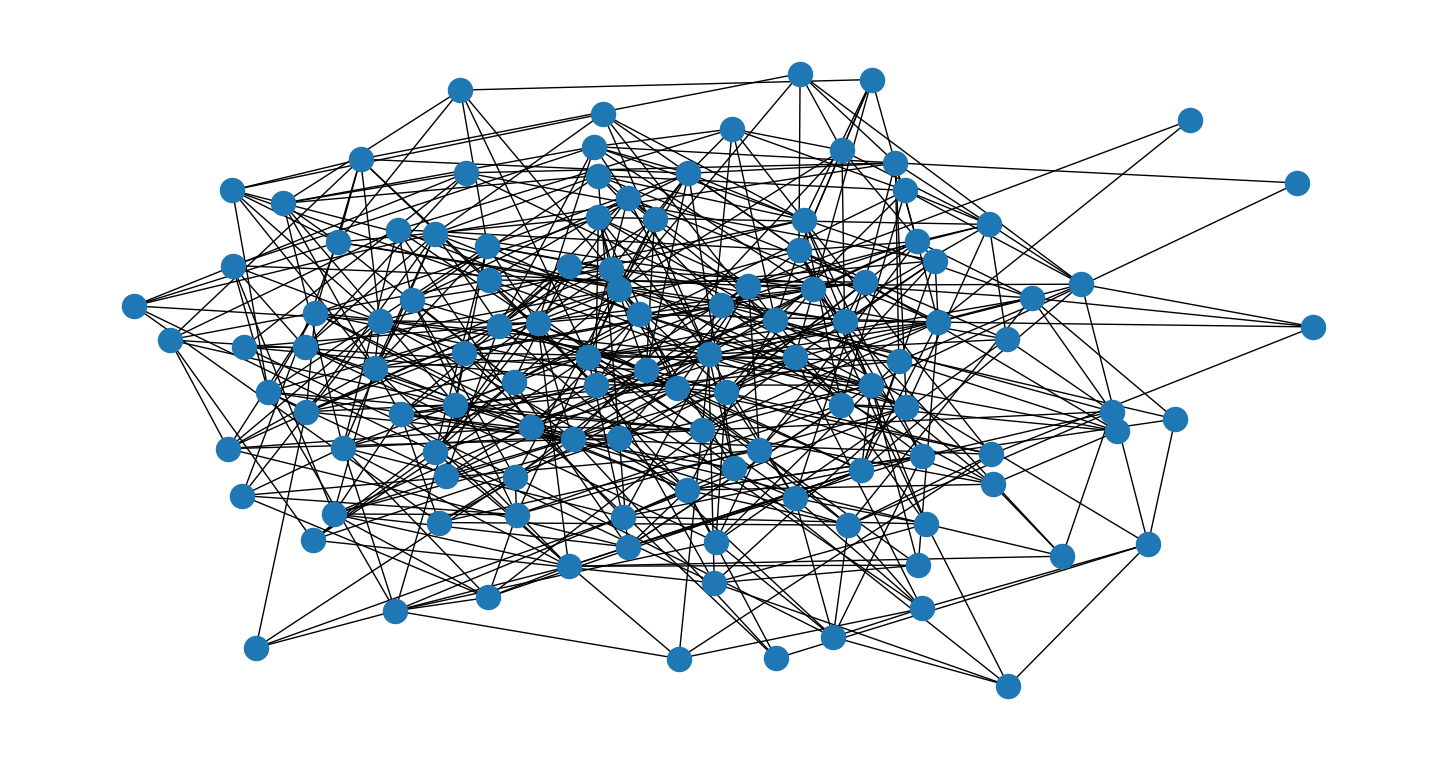
\includegraphics[width= \linewidth]{erdos_renyi}
		\caption{Azarosa}
		\label{fg:erdos_renyi}
	\end{subfigure}
	\begin{subfigure}[b]{0.32\textwidth}
		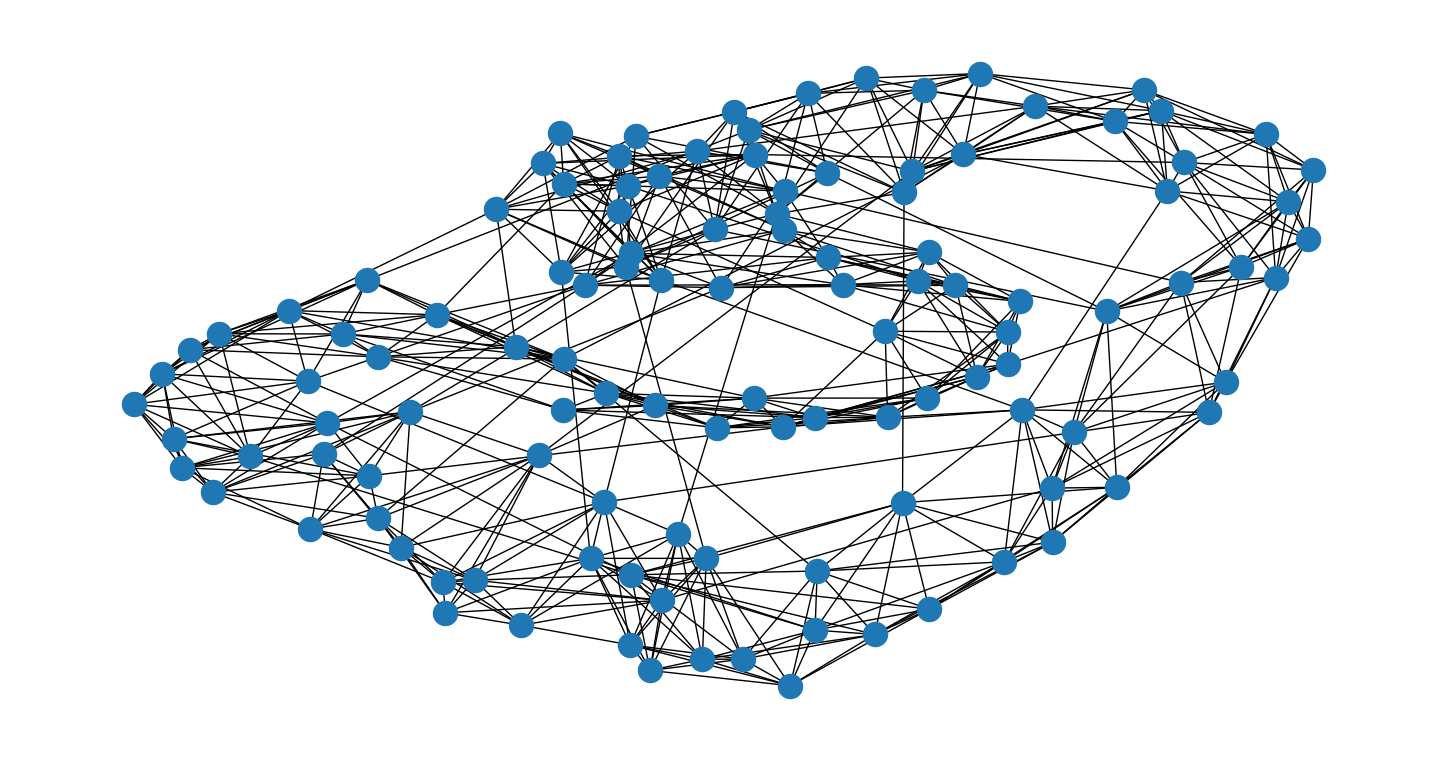
\includegraphics[width= \linewidth]{watts_strogatz}
		\caption{Pequeño mundo}
		\label{fg:watts_strogatz}
	\end{subfigure}
	\caption{Grafos prototípicos con número $n$ igual y $k$ similar a los de la red producto de las mediciones. 
	}
	\label{fg:prototípicas}
\end{figure}



\paragraph{Coeficientes de grafos propotípicos}

\begin{figure}[ht]
  \centering
  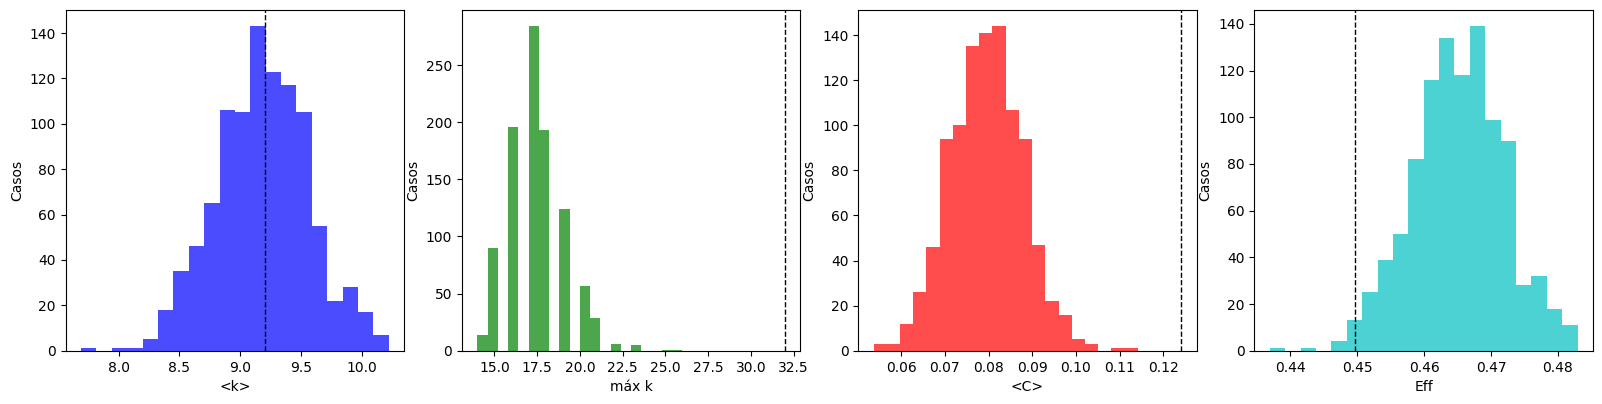
\includegraphics[width= \linewidth]{hist_poisson}
  \caption{Distribución de magnitudes que caracterizan las mil redes azarosas generadas.}
	\label{fg:hist_poisson}
\end{figure}



% \section{Discusión y conclusiones}

\printbibliography[title= Referencias, heading=bibintoc]

\end{document}
